Here, we explain some practical details in designing the experiments.

\subsection{Practical details in model implementation}
\label{sec:implementIssues}
The forward and adjoint equations are solved in a finite difference scheme using Euler's method. The time horizon $T$ is set to be 100 and $\Delta t = 0.01$. To save computation time, we assume that resources will only arrive at $t = 1, 2, 3, \ldots$, which makes $R(t)$ a piecewise function. The shape of $R(t)$ is shown in Fig. \ref{fig:resource}. Resource will only arrive after the reaction time $t_D$. Tests have been done during our implementation, and justify that a coarser discretization of resource mobilization has negligible influence on the qualitative  properties of the spreading process. In our implementation, we fix time delay $t_{ij}$ to $1.4$ instead of a random variable. The purpose of this setting is to speed up computation. In fact, this is not an important factor for the spreading process model in \cite{buzna2007efficient} and we can save a lot of computation time with this simplification.

\begin{figure}[!tb]	
	\centering
	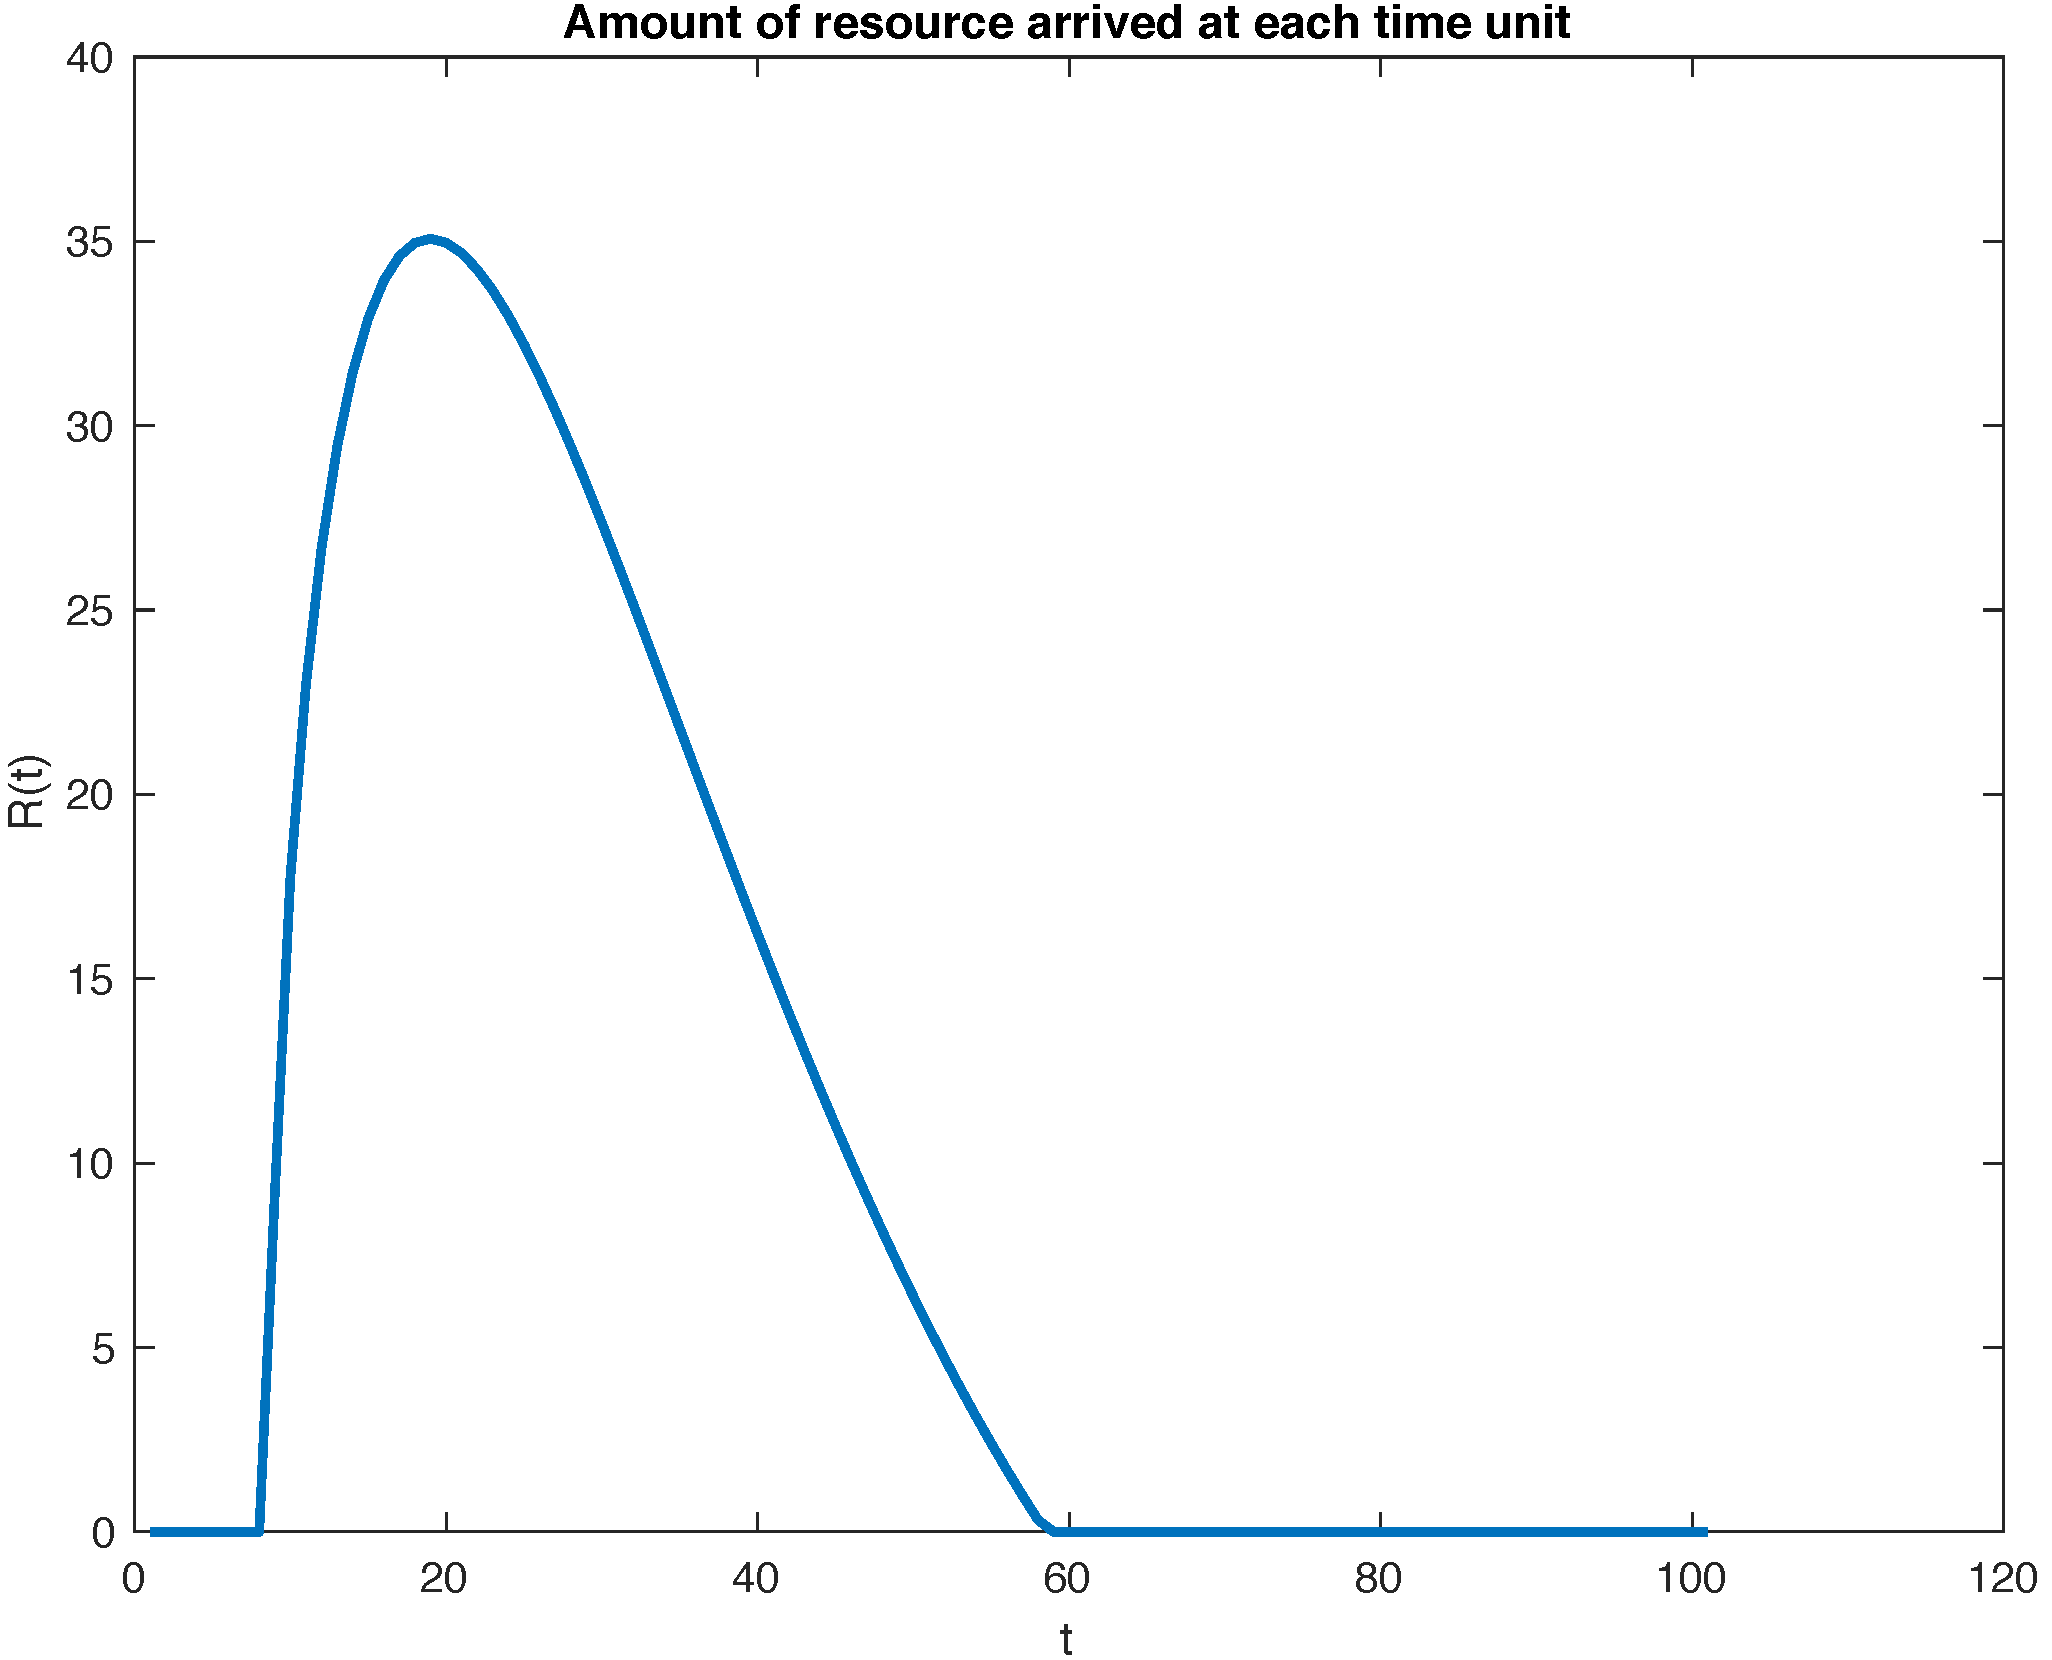
\includegraphics[height=80mm]{../figs/resource_small.pdf}
	\caption{Resource arriving at each time unit. $t_D=8$ and total resource is set to 1000.}
	\label{fig:resource}
\end{figure}

\subsection{Experiments setup}
\label{sec:experimentsSetup}
In this report, we first benchmarked our code with results in \cite{buzna2007efficient}. Then we studied effects of the choice of sigmoid coupling function in spreading model (Eq. (\ref{eq:sigmoid}) ) and replaced it with a linear function. Results showed that these two setups will lead to very different behaviors of the process. A sigmoid function with a large $\alpha$ prompts an easier spreading of disaster. 

After reproducing the results of original paper, we evaluate our optimization model. We choose two different objective functions (the first term in Eq. (\ref{eq:Lagrange}) ):  $\frac{1}{n}\sum_{i=1}^n x^{(i)}_T$ and $\sum_{i=1}^n \Theta(x_T^{(i)})$.  $\Theta(\cdot)$ is the same sigmoidal function as defined in Eq. (\ref{eq:sigmoid}). The first choice comes from that we want to minimize the averaging damage level of all nodes, while the second choice will lead to a minimization of total number of damaged nodes at time $T$. Detailed comparison of these two setups will be in Section \ref{sec:results}.